%\section{Wprowadzenie}
%\subsection{Machine learning}
%\subsection{Indukcyjne bazy danych}
%\subsection{Zastosowania}

\frame{
	\frametitle{Agenda}
	
Integracja technologii baz danych z nowoczesnymi metodami
indukcyjnego generowania wiedzy jest naturalnym kierunkiem rozwoju
system�w bazodanowych. Systemy nazywane czasem indukcyjnymi bazami
danych potrafi� odpowiedzie� nie tylko na pytania, dla kt�rych
odpowied� znajduje si� w bazie danych, ale r�wnie� na pytania,
kt�re wymagaj� zsyntetyzowania i zastosowania wiedzy,
wygenerowanej przez indukcyjne wnioskowanie z fakt�w z bazy danych
%i wcze�niejszej wiedzy~\cite{bib3}. Schemat typowej indukcyjnej
%bazy danych przedstawiony jest na rysunku~\ref{fig:inddb}.

%\begin{figure}[!ht]
%    \centering
%        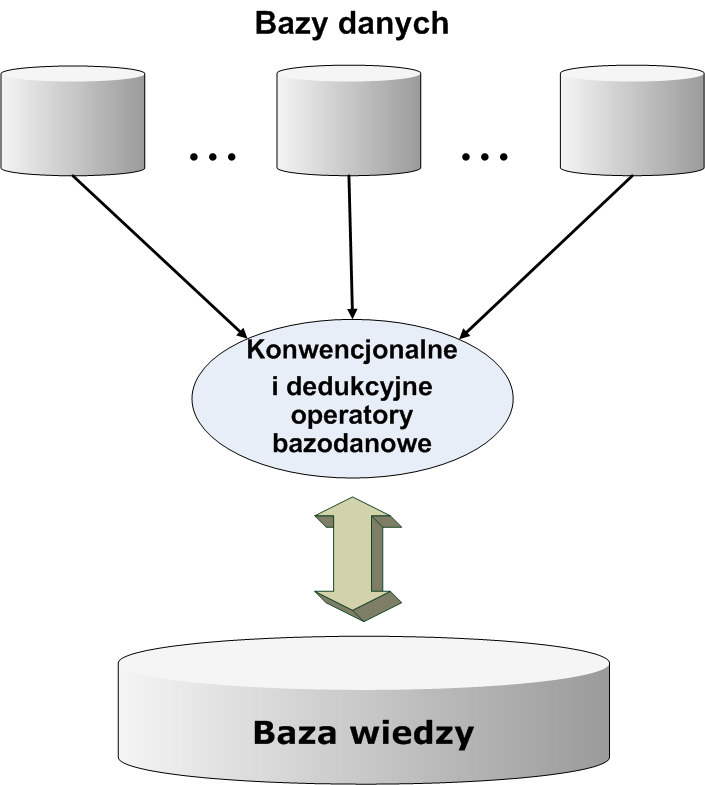
\includegraphics[width=\linewidth]{img/knowledge_mining.png}
    %\caption{Indukcyjna baza danych~\cite{bib2}}
%    \label{fig:inddb}
%\end{figure}

W pierwszej cz�ci pracy przedstawione zosta�y wybrane istniej�ce
�rodowiska wspieraj�ce uruchamianie algorytm�w uczenia maszynowego.
Dalej opisano za�o�enia, a~nast�pnie architektur� i wybrane aspekty
implementacji komponentowej realizacji indukcyjnej bazy danych --
platformy \emph{Salomon}.  Dzi�ki budowie modu�owej uda�o si� uzyska�
du�o wi�ksz� elastyczno�� systemu w stosunku do opisanych wcze�niej
rozwi�za�.  Ostatnia cz�� pracy prezentuje mo�liwo�ci wykorzystania
platformy do uczenia drzew decyzyjnych.

}